\documentclass[border=1pt]{standalone}
\usepackage{tikz}
\usetikzlibrary{arrows.meta,calc}

\begin{document}
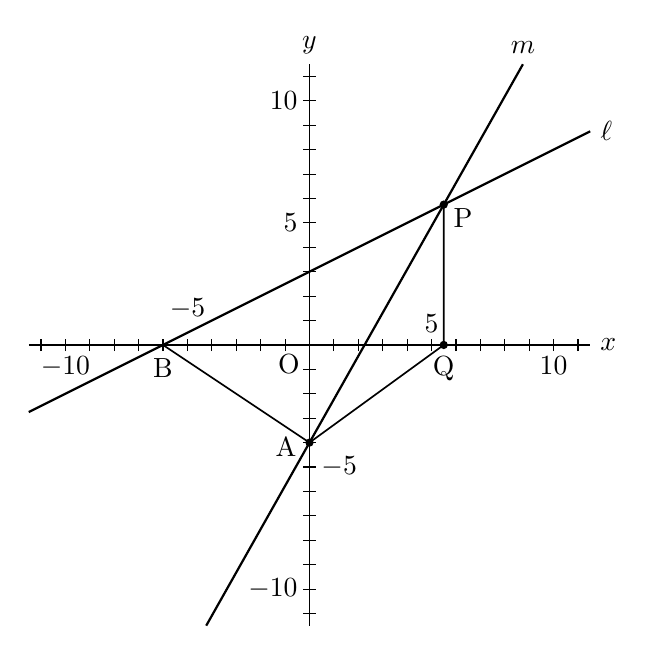
\begin{tikzpicture}[x=3.1mm, y=3.1mm]

    \pgfmathsetmacro{\xmax}{11.5}
    \pgfmathsetmacro{\ymax}{11.5}

    \pgfmathsetmacro{\xa}{22*\ymax/39+88/39}
    \pgfmathsetmacro{\xb}{-22*\ymax/39+88/39}

    \pgfmathsetmacro{\d}{0.25}

    % 座標軸
    \draw[semithick] (-\xmax,0) -- (\xmax,0) node[right] {$x$};
    \draw[semithick] (0,-\ymax) -- (0,\ymax) node[above] {$y$};
    
    % x軸・y軸の目盛り
    \foreach \x in {-11,-10,...,11} {
        \draw (\x,-\d) -- (\x,\d);
    }
    \foreach \y in {-11,-10,...,11} {
        \draw (-\d,\y) -- (\d,\y);
    }
    \foreach \x in {-10,10} {
        \node[below, outer sep=1pt] at (\x,0) {$\x$};
    }
    \foreach \y in {-10,5,10} {
        \node[left, outer sep=1pt] at (0,\y) {$\y$};
    }
    \node at (-5,0) [above, outer sep=6pt] {$-5$};
    \node at (5,0) [above, outer sep=1pt] {$5$};
    \node at (0,-5) [right, outer sep=1pt] {$-5$};


    % 直線 l: y = (1/2)x + 3 と 直線 m: y = (22/39)x + 88/39 を描画
    \draw[thick] (-\xmax,{-\xmax/2+3}) -- (\xmax,{\xmax/2+3}) node[right] {$\ell$};
    \draw[thick] (\xb,-\ymax) -- (\xa,\ymax) node[above] {$m$};

    % 原点
    \node[below left] at (0,0) {$\mathrm{O}$};
    
    % 点 A(0, -4)
    \fill (0,-4) circle (1.5pt) node[shift={(-8.5pt,-1.5pt)}] {$\mathrm{A}$}
    coordinate (A);
    
    % 点 B(-6, 0)
    \node[below, outer sep=1.5pt] at (-6,0) {$\mathrm{B}$};
    \coordinate (B) at (-6,0);
    
    % 点 P(5.5, 5.75)
    \fill (5.5,5.75) circle (1.5pt) node[shift={(7pt,-5pt)}] {$\mathrm{P}$}
    coordinate (P);

    % 点 Q(5.5, 0)
    \fill (5.5,0) circle (1.5pt) node[below, outer sep=1pt] {$\mathrm{Q}$}
    coordinate (Q);

    % BA，AQ，PQを描画
    \draw[semithick] (B)--(A)--(Q)--(P);
   
\end{tikzpicture}
\end{document}
